\documentclass[a4paper,14pt]{extarticle}
\usepackage[utf8]{inputenc}
\usepackage{helvet}
\usepackage{xcolor}
\usepackage{titlesec}
\usepackage{multicol}
\usepackage{geometry} 
\usepackage{wrapfig}
\usepackage{lipsum} 
\usepackage{pdfpages}

%TODO
%patch ideas logo
%patch ideas keep white but change font or bold
%new photo of ribbon, or (preferably) some schematic/diagram

\newgeometry{tmargin=0.5cm, bmargin=0.5cm, lmargin=0.5cm, rmargin=1cm} 
\renewcommand{\familydefault}{\sfdefault}
\definecolor{sectcolor}{rgb}{0.9,0.9,0.9}
\definecolor{Xcolor}{rgb}{0.91015625 , 0.015625, 0.015625}
\definecolor{Dcolor}{rgb}{0.0078125  , 0.                  , 0.41015625}
\definecolor{Acolor}{rgb}{0.03515625, 0.32421875, 0.01171875}
\definecolor{division_color}{rgb}{0.5,0.0,0.5}


\titleformat{\section}
  {\normalfont\LARGE\selectfont\bfseries}
  {\llap{\colorbox{sectcolor}{%
    \makebox[1.4cm][r]{%
      \makebox[0.7cm][l]{\thesection.\hfill}}%
      }\hspace{10pt}%
    }%
  }
  {0em}
  {}

\titleformat{\subsection}
  {\normalfont\Large\bfseries}
  {\llap{\colorbox{white}{%
    \makebox[1.4cm][r]{%
      \makebox[0.7cm][l]{\thesubsection\hfill}}%
      }\hspace{10pt}%
    }%
  }
  {0em}
  {}


\newlength\myboxwidth

\setlength{\myboxwidth}{\dimexpr\textwidth-0\fboxsep}
\definecolor{patchIdeasColor}{rgb}{0.3,0.3,0.3}

\begin{document}

\begin{flushright}
\includegraphics[scale=0.3]{./../../logo/Logo}
\end{flushright}
{\huge\textbf{SubShaper user manual}}\\*
\section*{What is SubShaper}
The module's name is a combination of two words, "Subharmonics" and "Waveshaper." This name reflects the two main functional parts of the module: waveshaping channels that add harmonics and clock dividers that introduce subharmonics.
\section*{Inputs and Outputs}

\begin{center}
\includegraphics[width=0.5\textwidth]{./NoA_SSH_colored_panel.png}
\end{center}
Module has \textbf{10 jacks}, divided into \textbf{2 groups}: on the left there are \textbf{4 common I/O} and on the right \textbf{3 modulation inputs} and \textbf{3 individual outputs}.

\begin{center}
\includegraphics[width=0.9\textwidth]{./SubShaper_Diagram_Colors_without_logo.png}
\end{center}

\section*{Behavior}

From left to right, waveshaper channels are:
\begin{itemize}
\item \textcolor{Xcolor}{X - crossover distortion}: This waveshaper simulates a class B amplifier that distorts the signal more as it gets quieter. "It can be considered the opposite of typical saturation/limiter distortion."\\
\includegraphics[width=9cm]{./crossover1.png}
\includegraphics[width=9cm]{./crossover2.png}
\item \textcolor{Dcolor}{D - frequency doubler}: As the name suggests, this waveshaper generates a wave at double the frequency of the input wave (at least for a sine wave). For a triangle wave, it generates a parabolic-like shape. This waveshaper is particularly useful for adding "soft" harmonics to the signal.\\
\includegraphics[width=9cm]{./sin_doubled.png}
\includegraphics[width=9cm]{./tri_doubled.png}
%\item \textcolor{Acolor}{A - absolute value}, it rectifies the signal. The knob goes from folding the top half bottom to letting the signal through to folding the bottom half up. Selectivelly change amplification of either half of the signal.\\
\item \textcolor{Acolor}{A - absolute value}, it allows you to selectively amplify and/or invert either half input wave. In it's middle position it let's the signal through, going counterclockwise it bends bottom half up to positive values while going clockwise bends top half down towards negative values.\\
\includegraphics[width=9cm]{./abs1.png}
\includegraphics[width=9cm]{./abs2.png}
\end{itemize}
\vspace{0.5cm}
\fcolorbox{patchIdeasColor}{patchIdeasColor}{
\begin{minipage}{\myboxwidth}
\textcolor{white}{(patch idea):  To better understand the effect of waveshapers we recommend sending audio to IN and listening to output from single channels individually}
\end{minipage}}
\\
\vspace{0.5cm}
\\
\fcolorbox{patchIdeasColor}{patchIdeasColor}{
\begin{minipage}{\myboxwidth}
\textcolor{white}{(patch idea):  Waveshaper channels can also be used independently for adding 3 new waveforms to your favourite VCO or LFO.}
\end{minipage}}
\vspace{0.5cm}
\\
Each waveshaper has a controllable parameter that can be modulated using CV (Control Voltage). Signal from modulation jack goes through attenuverter and gets summed with knob at the top. Modulation inputs accept audio rate modulation allowing for many interesting effects, including MI Warps like wave mixing or self modulation where one waveshaper channel modulates the other.
\\
Note that outputs from waveshapers are not influenced by clock divisions.
\vspace{0.5cm}
\\
\fcolorbox{patchIdeasColor}{patchIdeasColor}{
\begin{minipage}{\myboxwidth}
\textcolor{white}{(patch idea):  Try using output of abs to modulate doubler. Change modulation depth and polarity by rotating doubler attenuverter. You can keep it simple or go wild with multiple feedback loops.}
\end{minipage}}
\vspace{0.5cm}
\\
Clock divisions can be set for each channel using the \textcolor{division_color}{slide switches}. There are \textbf{2 banks} of selections, one for \textbf{simpler, more octave} sounds, one for more \textbf{complicated harmonic structures}. All 3 switches have to work in the same bank. The clock dividers are stateless. It means that any switch changes immediately reflected at the output. If one switches from one clock division that was off to the other that was on results show up instantly, not waiting for next clock period. It's important as it keeps channels in sync and predictable when live patching.
\vspace{0.5cm}
\\
\fcolorbox{patchIdeasColor}{patchIdeasColor}{
\begin{minipage}{\myboxwidth}
\textcolor{white}{(patch idea): AUX doesn't use switches so comparing it to OUT is good starting point to grasp inner working of dividers. For Simplicity we recommend setting 2 channels to off and fill to Ø to start with one channel at the time.}
\end{minipage}}
\vspace{0.5cm}
\\
\textcolor{division_color}{Clock dividers} get clocked by CLK that is normalised to IN. Thanks to that normalisation subharmonics can be generated with just default internal routing. This normalisation can be broken by inserting any jack into CLK. It's useful for low frequency waveshaper switching, ring modulating one oscillator with another or delaying/phase shifting square wave from VCO. Logic high threshold is set to around 1.2V, counters get advanced on every rising edge of input clock/gate. Thanks to that module can be patched with both gates and triggers.
\vspace{0.5cm}
\\
\fcolorbox{patchIdeasColor}{patchIdeasColor}{
\begin{minipage}{\myboxwidth}
\textcolor{white}{(patch idea): Try enabling just one channel (like in previous patch) and patch slow LFO into CLK. You'll hear signal being on and off. By speeding up LFO one gets into ringmod like terythory. }
\end{minipage}}
\vspace{0.5cm}
\\
Clock dividers can be on or off, and there may be instances when all channels are turned off and aligned, resulting in no audio output. This can be undesirable, particularly when using slow modulation clocks.  o address this, we have introduced the \textbf{FILL switch}. This switch allows you to choose what happens during periods of silence in the output. You can select to fill the silence with either the X channel (marked as A on the first revision of panels), the D channel (marked as B on the first revision of panels),  the A channel (marked as C on the first revision of panels) or modes 3 or 4. The 3 and 4 modes require further explanation. In the 3 mode, the gaps will be filled alternately with \textcolor{Xcolor}{X}, \textcolor{Dcolor}{D}, \textcolor{Acolor}{A},\textcolor{Xcolor}{X}, \textcolor{Dcolor}{D}, \textcolor{Acolor}{A}, repeating in that sequence. In the 4 mode, silence will be reintroduced at the output every fourth division, following the pattern \textcolor{Xcolor}{X}, \textcolor{Dcolor}{D}, \textcolor{Acolor}{A}, Ø, \textcolor{Xcolor}{X}, \textcolor{Dcolor}{D}, \textcolor{Acolor}{A}, Ø, and so on.

\section*{Installation}
SSH requires standard eurorack power supply, on 10 pin IDC connector. The red stripe of the ribbon cable (-12V side) must be oriented to the bottom of the module, in the direction when inner PCB ends, in the direction of jacks. In case of big resistance during connection of power supply connector should
be supported from other side, to avoid applying excessive pressure to PCB and damaging it. Module draws up to \textbf{100mA} of current from both supply rails. Module should be screwed with 4 bolts into compatible eurorack case prior to any patching, otherwise damage may occur due to excessive forces. Nylon washers are recommended if one wishes to not scratch powder coating on panel, so called rackrash.
\\
%\begin{center}
%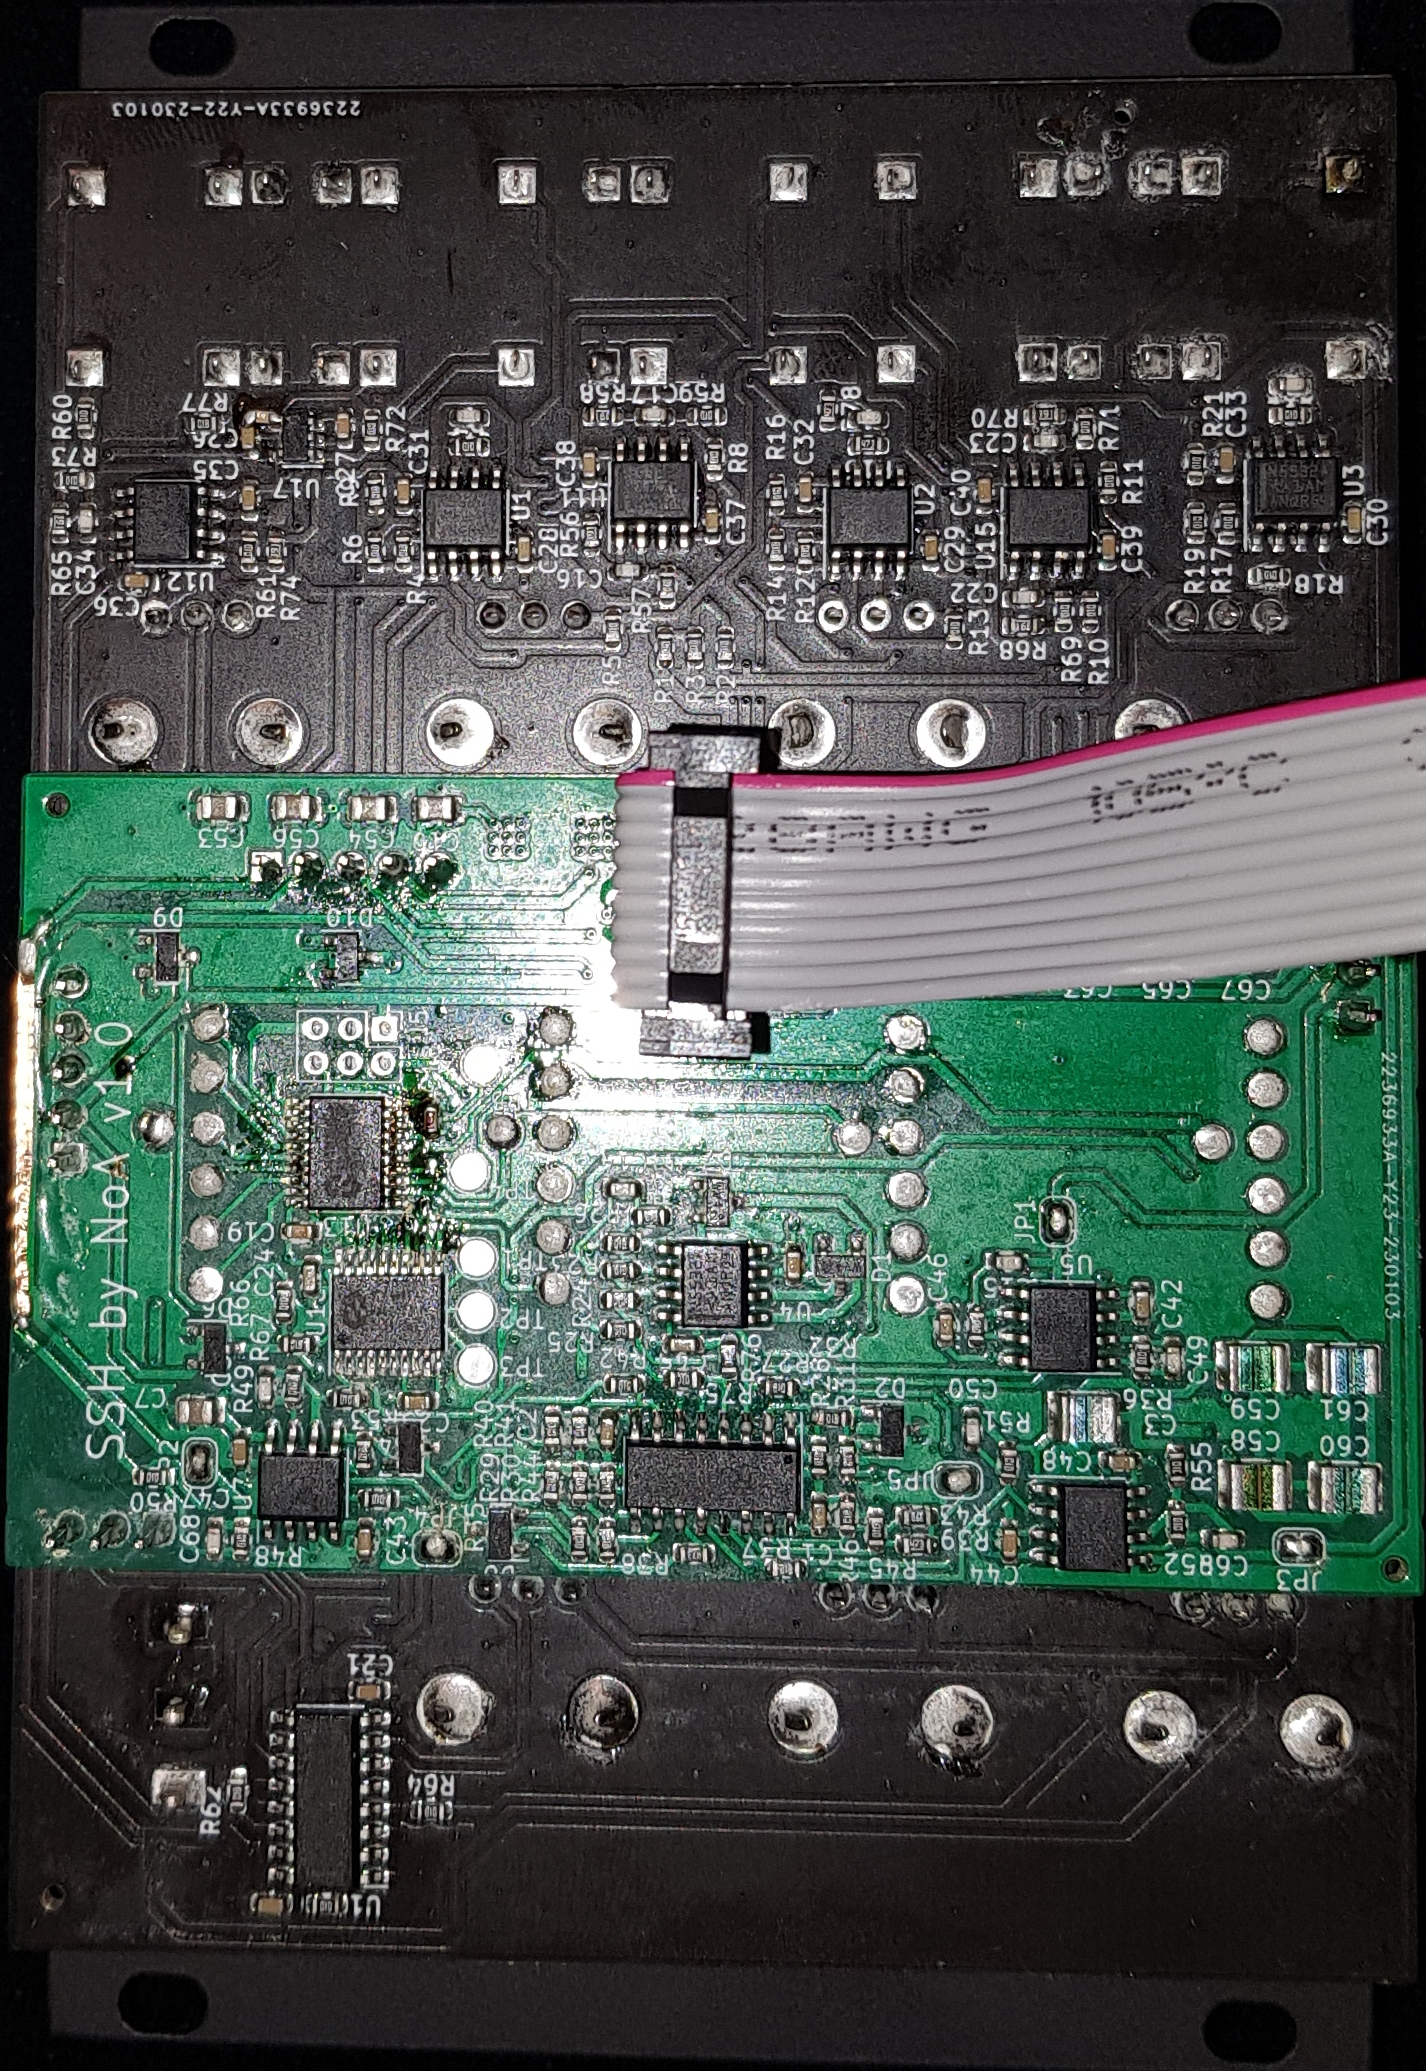
\includegraphics[width=0.5\textwidth,angle=90]{./tasiemka.jpg}
%\end{center}

\section*{Warranty}
Module is covered with 2-years warranty since day of purchase. Warranty does not cover malfunction caused by incorrect use (such as reverse power connection, excessive voltage levels, bad weather conditions, or physical damages). This warranty covers defects resulting from the manufacturing of this product only. Before sending module to service, please contact us at support@noiseofantimatter.com\\
If your warranty expired or malfunction is result of users actions feel free to contact us for out-of-warranty service and/or self-service help.
\section*{EMC compliance}
Noise of antimatter verifies that a properly constructed modular system, adhering to the Doepfer standard, based on cases, power supplies, power distribution boards and a coherent selection of modules, available from other manufacturers meets the requirements defined by international certification bodies.\\

In the paragraphs that follow, Device refers to the Eurorack module, properly installed, powered, and patched as part of a system.\\
This device complies with Part 15 of the FCC Rules. Operation is subject to the following two conditions: (1) this device may not cause harmful interference, and (2) this device must accept any interference received, including interference that may cause undesired operation.\\
Changes / modifications could void the user’s authority to operate the equipment.
\\
This device meets the requirements of the following standards:
\begin{itemize}
\item    EN55032. Electromagnetic compatibility of multimedia equipment. Emission requirements.
\item    EN55103-2. Electromagnetic compatibility - Product family standard for audio, video, audio-visual and entertainment lighting control apparatus for professional use.
\item    EN61000-3-2. Limits for harmonic current emissions (equipment input current $\leq$ 16 A per phase).
\item    EN61000-3-3. Limitation of voltage changes, voltage fluctuations and flicker in public low-voltage supply systems, for equipment with rated current $\leq$ 16 A per phase and not subject to conditional connection.
\item    EN62311. Assessment of electronic and electrical equipment related to human exposure restrictions for electromagnetic fields (0 Hz - 300 GHz).
\end{itemize}

\end{document}